\chapter{Metabolismo microbiano e biofilmes}\label{ch:b2:microbial-metabolism}

Encha um cilindro de vidro com lama de lagoa, um pouco de papel
picado, uma gema de ovo e água, e deixe-o no parapeito de uma janela.
Em poucas semanas, ele se estratifica em faixas coloridas: algas verdes
no topo, uma camada cor de ferrugem, uma faixa púrpura, uma verde mais
abaixo e lama negra de sulfeto no fundo. Nada foi acrescentado além da
luz. Cada faixa é uma população que vive de uma química diferente ---
de oxigênio, de nitrato, de sulfato, de sulfeto, de hidrogênio --- e
cada uma alimenta a seguinte. A coluna é o mundo microbiano em
miniatura: células que obtêm sua energia de quase qualquer par de
substâncias capazes de trocar elétrons e que, juntas, fazem funcionar
os ciclos químicos do planeta. Este capítulo expõe a lógica dessa
energética, a cinética do crescimento microbiano e a vida coletiva dos
micróbios sobre superfícies, que é como a maioria deles de fato vive.

\section{Maneiras de ganhar a vida}

\begin{definition}[Tipos tróficos]\label{def:b2:microbial-metabolism:trophic}
\index{quimiotrófico}\index{fototrófico}\index{litotrófico}\index{organotrófico}
Um organismo é classificado por três respostas. Sua \emph{fonte de
energia}: a luz (\emph{fototrófico}) ou reações químicas
(\emph{quimiotrófico}). Sua \emph{fonte de elétrons}: substâncias
inorgânicas --- $\mathrm{H_2}$,
$\mathrm{H_2S}$, $\mathrm{NH_4^+}$, $\mathrm{Fe^{2+}}$, água ---
(\emph{litotrófico}) ou moléculas orgânicas (\emph{organotrófico}). Sua
\emph{fonte de carbono}: o $\mathrm{CO_2}$ (\emph{autotrófico}) ou o
carbono orgânico (\emph{heterotrófico}). As plantas e as cianobactérias
são fotolitoautotróficas; os animais, os fungos e \emph{E.~coli} são
quimiorganoheterotróficos; as bactérias nitrificantes e as oxidantes
de enxofre são quimiolitoautotróficas: produzem sua matéria orgânica a
partir do $\mathrm{CO_2}$ com a energia tirada da oxidação de
minerais, no escuro. Quase todas as combinações existem em algum lugar
entre os \omterm{def:b2:unicellular-diversity:prokaryote}{procariotos}; os eucariotos ocupam apenas duas.
\end{definition}

\begin{theorem}[A energia de um par redox]\label{thm:b2:microbial-metabolism:redox}
\index{potencial redox}\index{torre de elétrons}
Todo metabolismo que fornece energia desloca elétrons de um par
\emph{doador} para um par \emph{aceptor}. Cada par tem um potencial
padrão $E^{\circ\prime}$ (a pH 7): quanto mais negativo, mais
facilmente cede elétrons. Transferir $n$ mols de elétrons de um doador
a $E_d$ para um aceptor a $E_a$ libera uma energia livre padrão
\[
\Delta G^{\circ\prime} = -\,n F\,(E_a - E_d), \qquad F = \qty{96.5}{kJ/V/mol},
\]
de modo que o rendimento é proporcional à distância vertical entre os
dois pares na \emph{\omterm{thm:b2:microbial-metabolism:redox}{torre de elétrons}}. Com
$\mathrm{O_2/H_2O}$ a \qty{+0.82}{V} e $\mathrm{CO_2}$/glicose a
\qty{-0.43}{V}, os 24 elétrons de uma molécula de glicose fornecem
$24\times 96.5\times 1.25 = \qty{2900}{kJ/mol}$; entregues ao sulfato
($\mathrm{SO_4^{2-}/H_2S}$, \qty{-0.22}{V}), os mesmos elétrons
fornecem apenas $24\times 96.5\times 0.21 = \qty{490}{kJ/mol}$.
\end{theorem}
\begin{proof}
Para a reação doador$_{\text{red}}$ + aceptor$_{\text{ox}}$
$\to$ doador$_{\text{ox}}$ + aceptor$_{\text{red}}$, a variação de
energia livre é o trabalho realizado por $n$ mols de carga eletrônica
$nF$ que caem pela diferença de potencial $E_a - E_d$, com a convenção
de sinal de que uma transferência espontânea (elétrons em direção ao
par mais positivo) tem $\Delta G < 0$. É a relação de Nernst do volume
do Ano 1 aplicada a duas semirreações.
\end{proof}

\begin{omfigure}
\begin{tikzpicture}[every node/.style={font=\scriptsize}, y=6cm]
  \draw[thick, ->] (0,-0.55) -- (0,0.95) node[above] {$E^{\circ\prime}$ (V)};
  \foreach \v in {-0.4,-0.2,0,0.2,0.4,0.6,0.8} \draw (-0.08,\v) -- (0.08,\v) node[right, xshift=0.05cm] {\v};
  % donors on the right: value/label position/text
  \foreach \v/\y/\l in {-0.43/-0.49/{$\mathrm{CO_2}$/glucose}, -0.42/-0.40/{$2\mathrm{H^+/H_2}$}, -0.32/-0.31/{$\mathrm{NAD^+/NADH}$}, -0.27/-0.22/{$\mathrm{S^0/H_2S}$}, 0.03/0.03/{fumarato/succinato}, 0.34/0.34/{$\mathrm{NO_2^-/NH_4^+}$}}
    { \draw[omDef, thick] (0.8,\v) -- (1.6,\v); \draw[omDef] (1.6,\v) -- (1.85,\y); \node[omDef, anchor=west] at (1.9,\y) {\l}; }
  % acceptors on the left
  \foreach \v/\y/\l in {-0.24/-0.29/{$\mathrm{CO_2/CH_4}$}, -0.22/-0.17/{$\mathrm{SO_4^{2-}/H_2S}$}, 0.43/0.43/{$\mathrm{NO_3^-/NO_2^-}$}, 0.74/0.69/{$\mathrm{NO_3^-/N_2}$}, 0.77/0.77/{$\mathrm{Fe^{3+}/Fe^{2+}}$}, 0.82/0.86/{$\mathrm{O_2/H_2O}$}}
    { \draw[omThm, thick] (-1.6,\v) -- (-0.8,\v); \draw[omThm] (-1.6,\v) -- (-1.85,\y); \node[omThm, anchor=east] at (-1.9,\y) {\l}; }
  \node[omThm, anchor=south] at (-2.4,0.93) {aceptores};
  \node[omDef, anchor=south] at (2.4,0.93) {doadores};
  % arrows showing two metabolisms
  \draw[->, very thick, omExo!80!black] (4.9,-0.43) -- (4.9,0.80);
  \node[anchor=west, align=left] at (5.0,0.2) {respiração aeróbia\\da glicose: \qty{1.25}{V},\\\qty{2900}{kJ/mol}};
  \draw[->, very thick, omProp] (4.2,-0.43) -- (4.2,-0.24);
  \node[anchor=north, align=center] at (4.2,-0.52) {redução do sulfato:\\\qty{0.21}{V}, \qty{490}{kJ/mol}};
  \draw[dashed, gray] (3.5,-0.43) -- (4.9,-0.43);
  \draw[dashed, gray] (3.5,0.82) -- (4.9,0.82);
  \draw[dashed, gray] (3.5,-0.22) -- (4.2,-0.22);
\end{tikzpicture}

{\small A \omterm{thm:b2:microbial-metabolism:redox}{torre de elétrons}. Os doadores (azul) estão dispostos em seus
potenciais padrão; os aceptores (vermelho), do mesmo modo. Um
metabolismo é uma queda de um doador até um aceptor situado acima dele,
e seu rendimento energético é proporcional à altura da queda: da
glicose ao oxigênio é uma queda longa; da glicose ao sulfato, uma
queda curta.}
\end{omfigure}

\begin{proposition}[Quimiolitotrofia]\label{prop:b2:microbial-metabolism:lithotrophy}
\index{quimiolitotrofia}\index{nitrificação}
Algumas bactérias tiram toda a sua energia de oxidações inorgânicas,
usando o oxigênio (ou o nitrato) como aceptor, e fixam o
$\mathrm{CO_2}$ com o ATP e o poder redutor assim obtidos.
\emph{Nitrificantes}: as oxidantes de amônio (\emph{Nitrosomonas})
transformam o $\mathrm{NH_4^+}$ em nitrito
($\Delta G^{\circ\prime} = \qty{-275}{kJ/mol}$), as oxidantes de
nitrito (\emph{Nitrobacter}) transformam o nitrito em nitrato
(\qty{-74}{kJ/mol}); juntas, convertem o amônio da decomposição no
nitrato que as plantas absorvem (\cref{ch:b2:biogeochemical-cycles}).
As \emph{oxidantes de enxofre} (\emph{Thiobacillus}, \emph{Beggiatoa})
oxidam o $\mathrm{H_2S}$ a enxofre e sulfato; as \emph{oxidantes de
ferro} oxidam o $\mathrm{Fe^{2+}}$ a ferrugem; as \emph{oxidantes de
hidrogênio} queimam o
$\mathrm{H_2}$. Como seus doadores de elétrons ficam no alto da torre,
o rendimento por molécula é pequeno, e como esses doadores são
redutores mais fracos que o NADH, elas precisam gastar energia para
empurrar elétrons \emph{ladeira acima} a fim de produzir o NADH de que
a fixação do carbono necessita: uma nitrificante oxida cerca de trinta
íons amônio para fixar um $\mathrm{CO_2}$, e cresce devagar.
\end{proposition}
\begin{proof}[Evidências]
Winogradsky (1887--1890) cultivou bactérias sulfurosas filamentosas
numa gota de água na qual deixava o sulfeto difundir-se de um lado e
o ar do outro: elas se reuniam na fronteira, acumulavam glóbulos de
enxofre e os consumiam quando o sulfeto era cortado. Depois, isolou
bactérias nitrificantes num meio puramente mineral, contendo amônio e
nenhum carbono orgânico, no qual elas cresciam e produziam nitrato ---
a primeira demonstração de que a vida pode ser construída a partir do
$\mathrm{CO_2}$ e da energia de uma reação inorgânica, sem luz. Ele
chamou isso de quimiossíntese.
\end{proof}

\begin{omfigure}
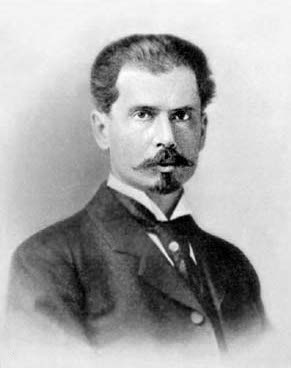
\includegraphics[width=0.26\linewidth]{images/book4/winogradsky.jpg}\hspace{0.05\linewidth}
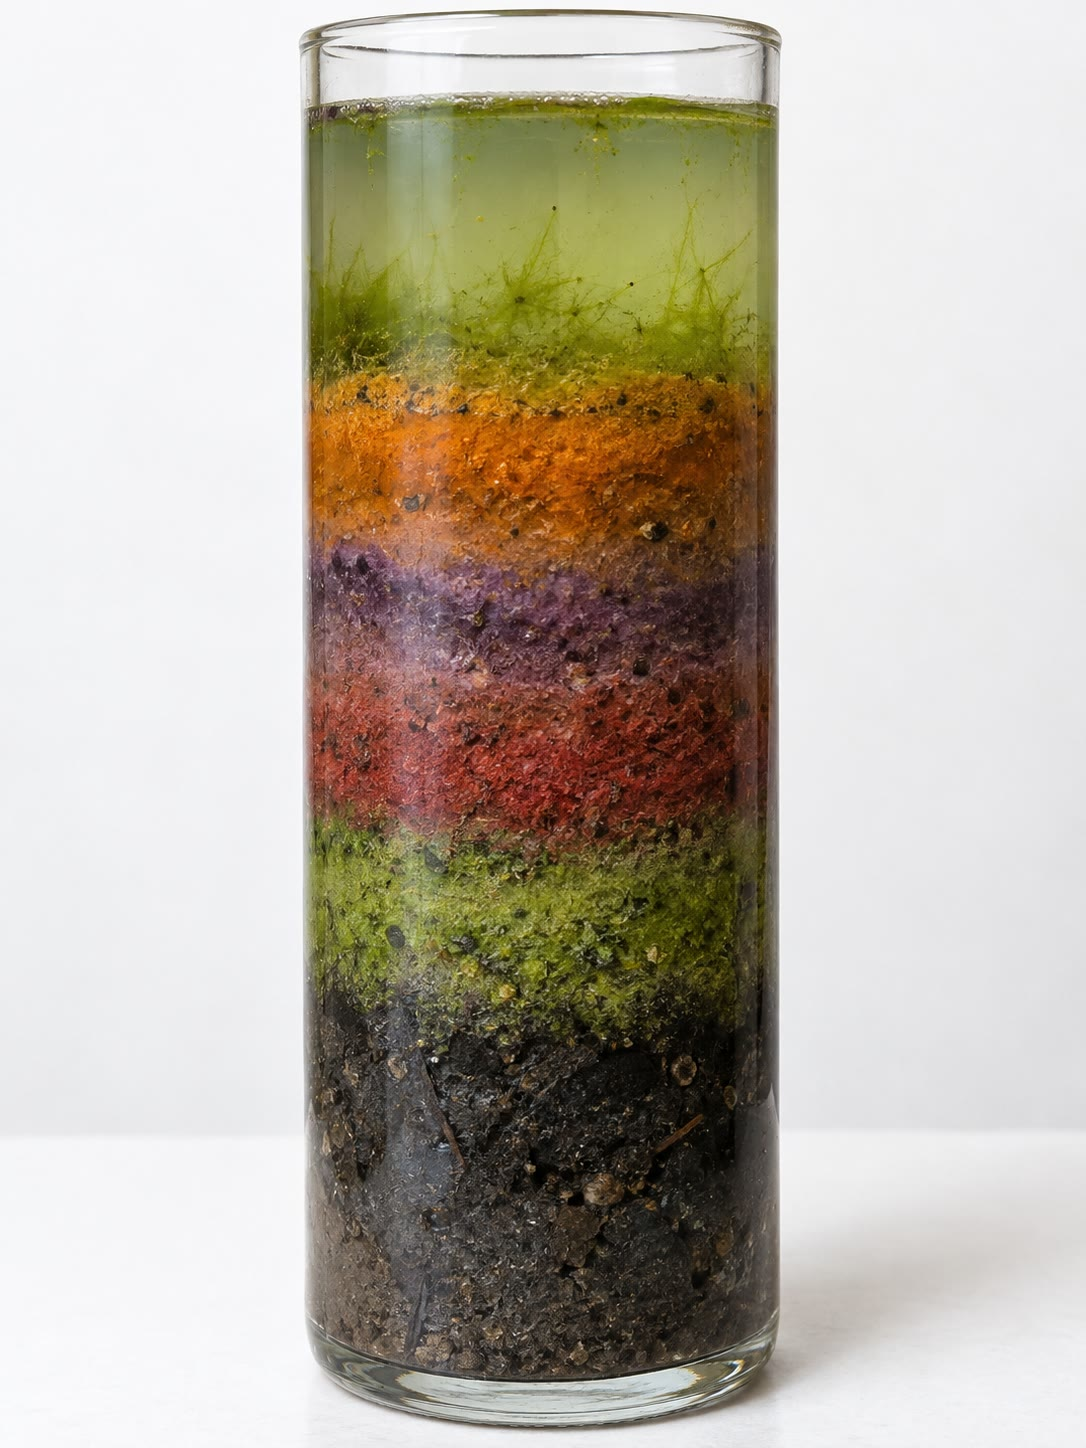
\includegraphics[width=0.30\linewidth]{images/book4/ai/b4-02-winogradsky-column.jpg}

{\small Sergei Winogradsky, que descobriu a \omterm{def:b2:microbial-metabolism:trophic}{quimiolitotrofia}, e a
coluna que leva seu nome: um cilindro de lama e água que, sob a luz, se
estratifica em faixas de algas, de oxidantes de ferro e de enxofre, de
bactérias sulfurosas púrpuras e verdes, e de redutoras de sulfato na
lama negra.}
\end{omfigure}

\begin{definition}[Fotossíntese anoxigênica]\label{def:b2:microbial-metabolism:anoxygenic}
\index{fotossíntese anoxigênica}
As bactérias púrpuras e verdes fazem fotossíntese com um único
fotossistema e uma bacterioclorofila que absorve no infravermelho
próximo, usando $\mathrm{H_2S}$, $\mathrm{H_2}$ ou ácidos orgânicos
como doadores de elétrons em vez da água: liberam enxofre ou sulfato,
nunca oxigênio, e precisam de luz de comprimentos de onda que
atravessam a camada verde e de cianobactérias acima delas. As
bactérias sulfurosas púrpuras crescem, por isso, na faixa púrpura da
coluna de Winogradsky, exatamente onde o sulfeto que vem de baixo
encontra a luz que vem de cima; as bactérias sulfurosas verdes, que
toleram mais sulfeto e menos luz, crescem logo abaixo delas. A
fotossíntese oxigênica, com seus dois fotossistemas em série, é uma
invenção posterior de uma linhagem --- as cianobactérias --- que
aprendeu a tirar elétrons da água.
\end{definition}

\section{Respirações anaeróbias e fermentações}

\begin{definition}[Respiração anaeróbia]\label{def:b2:microbial-metabolism:anaerobic}
\index{respiração anaeróbia}\index{desnitrificação}\index{redução do sulfato}\index{metanogênese}
A \emph{respiração anaeróbia} é uma respiração --- uma cadeia
transportadora de elétrons que bombeia prótons e produz ATP por
quimiosmose --- com um aceptor terminal diferente do oxigênio. Os
\emph{desnitrificantes} (\emph{Pseudomonas}, \emph{Paracoccus})
reduzem o nitrato a nitrito, óxido nítrico, óxido nitroso e por fim
$\mathrm{N_2}$, que escapa para o ar; usam sua cadeia aeróbia com
algumas enzimas a mais e passam ao nitrato apenas quando o oxigênio
acaba. Os \emph{redutores de sulfato} (\emph{Desulfovibrio}) reduzem o
sulfato a sulfeto, enegrecem a lama com sulfeto de ferro e lhe dão
seu cheiro. Os \emph{metanogênicos},
que são arqueias, reduzem o $\mathrm{CO_2}$ com $\mathrm{H_2}$ a
metano ($4\mathrm{H_2} + \mathrm{CO_2} \to \mathrm{CH_4} +
2\mathrm{H_2O}$, $\Delta G^{\circ\prime} = \qty{-131}{kJ/mol}$), ou
quebram o acetato em metano e $\mathrm{CO_2}$; o oxigênio os mata, e
eles vivem no rúmen das vacas, nos arrozais, nos pântanos e nos
aterros sanitários, de onde liberam um gás de efeito estufa que é
objeto do \cref{ch:b2:global-change}. Os óxidos de ferro e de manganês servem a outros
grupos. O volume do Ano 1 tratou o oxigênio como \emph{o} aceptor;
durante a maior parte da história da Terra, e em todo sedimento hoje,
ele é apenas o primeiro de uma série.
\end{definition}

\begin{proposition}[A sequência dos aceptores num sedimento]\label{prop:b2:microbial-metabolism:sequence}
Descendo num sedimento encharcado, os aceptores de elétrons se esgotam
na ordem da energia que fornecem: o oxigênio nos primeiros milímetros,
depois o nitrato, depois os óxidos de manganês e de ferro, depois o
sulfato e, por fim, o $\mathrm{CO_2}$ (\omterm{def:b2:microbial-metabolism:anaerobic}{metanogênese}) na camada anóxica
mais profunda. A ordem é a da torre: em cada profundidade, os
organismos que usam o melhor aceptor restante crescem mais depressa,
superam os demais na competição pelos doadores orgânicos e esgotam
seu aceptor antes que o grupo seguinte assuma. No mar, onde o sulfato
é abundante (\qty{28}{mmol/L}), a zona do sulfato é espessa e a
\omterm{def:b2:microbial-metabolism:anaerobic}{metanogênese} começa apenas a alguns metros de profundidade; num
pântano de água doce, pobre em sulfato, o metano se forma logo abaixo
da superfície.
\end{proposition}

\begin{omfigure}
\begin{tikzpicture}[every node/.style={font=\scriptsize}]
  \fill[omDef!8] (0,0) rectangle (4,0.6);
  \node at (2,0.3) {água};
  \fill[omExo!35] (0,-0.5) rectangle (4,0);
  \fill[omProp!25] (0,-1.3) rectangle (4,-0.5);
  \fill[omProp!45] (0,-2.0) rectangle (4,-1.3);
  \fill[gray!50] (0,-3.4) rectangle (4,-2.0);
  \fill[black!75] (0,-4.4) rectangle (4,-3.4);
  \draw[thick] (0,0.6) -- (0,-4.4); \draw[thick] (4,0.6) -- (4,-4.4);
  \draw[thick] (0,0) -- (4,0);
  \node[anchor=west, align=left] at (4.2,-0.25) {respiração do oxigênio: $\mathrm{O_2 \to H_2O}$ --- \qty{2.9}{MJ} por glicose};
  \node[anchor=west, align=left] at (4.2,-0.9) {redução do nitrato: $\mathrm{NO_3^- \to N_2}$ --- \qty{2.7}{MJ}};
  \node[anchor=west, align=left] at (4.2,-1.65) {redução do manganês e do ferro: $\mathrm{Fe^{3+} \to Fe^{2+}}$};
  \node[anchor=west, align=left, white] at (0.1,-2.7) {};
  \node[anchor=west, align=left] at (4.2,-2.7) {redução do sulfato: $\mathrm{SO_4^{2-} \to H_2S}$ --- \qty{0.5}{MJ}};
  \node[anchor=west, align=left] at (4.2,-3.9) {metanogênese: $\mathrm{CO_2 \to CH_4}$ --- \qty{0.4}{MJ}};
  \draw[->, thick] (-0.5,0) -- (-0.5,-4.4) node[below] {profundidade};
  \node[anchor=east] at (-0.6,-0.25) {mm};
  \node[anchor=east] at (-0.6,-2.7) {de cm a m};
\end{tikzpicture}

{\small A sucessão dos aceptores de elétrons com a profundidade num
sedimento, na ordem da energia que cada um fornece por glicose. Os
organismos de cada zona superam os da zona seguinte na competição pela
matéria orgânica até que seu aceptor se esgote.}
\end{omfigure}

\begin{definition}[A fermentação revisitada]\label{def:b2:microbial-metabolism:fermentation}
\index{fermentação!microbiana}
Uma \emph{fermentação} não usa aceptor externo: o substrato orgânico
é quebrado num produto mais oxidado e num mais reduzido, o ATP é
produzido apenas por fosforilação em nível de substrato, e o NADH da
glicólise é reoxidado pela redução de um metabólito. As leveduras
produzem etanol e $\mathrm{CO_2}$; as bactérias lácticas produzem
lactato (iogurte, chucrute, músculos doloridos); \emph{E.~coli}
produz uma mistura de ácidos, etanol e gases; os clostrídios produzem
butirato, butanol e acetona; as propionibactérias produzem o
propionato e o $\mathrm{CO_2}$ do queijo suíço. O rendimento é de dois
ATP por glicose contra cerca de trinta na respiração, de modo que um
fermentador precisa processar quinze vezes mais açúcar para o mesmo
crescimento, e seus produtos --- ácidos, álcool --- envenenam seu
próprio meio: as fermentações conservam os alimentos porque o
fermentador torna o alimento inabitável, inclusive para si mesmo.
\end{definition}

\begin{example}[Sintrofia: viver das sobras]\label{ex:b2:microbial-metabolism:syntrophy}
Num sedimento anóxico, os fermentadores deixam para trás acetato,
propionato, butirato e $\mathrm{H_2}$. Oxidar o propionato a acetato e
$\mathrm{H_2}$ tem uma energia livre padrão \emph{positiva}
(\qty{+76}{kJ/mol}) e é impossível --- a menos que um metanogênico
vizinho consuma o hidrogênio tão depressa quanto ele se forma,
mantendo sua pressão parcial abaixo de \qty{1e-4}{atm}, valor em que a
reação se torna exergônica. Nenhum dos parceiros consegue crescer
sozinho em propionato; juntos, eles o transformam em metano. Essa
\emph{transferência interespecífica de hidrogênio} explica por que a
digestão anaeróbia é sempre obra de um consórcio, e por que a arqueia
e sua parceira bacteriana são frequentemente encontradas encostadas
uma na outra.
\end{example}

\section{Crescimento sobre um substrato}

\begin{theorem}[Lei de Monod]\label{thm:b2:microbial-metabolism:monod}
\index{equação de Monod}\index{coeficiente de rendimento}
Uma população que cresce sobre um único substrato limitante, de
concentração $S$, tem uma taxa específica de crescimento
\[
\mu = \mu_{\max}\,\frac{S}{K_s + S}, \qquad \frac{\mathrm{d}X}{\mathrm{d}t} = \mu X,
\]
em que $X$ é a concentração de biomassa, $\mu_{\max}$ a taxa máxima
(o inverso do menor \omterm{def:b2:unicellular-diversity:division}{tempo de geração} dividido por
$\ln 2$) e $K_s$ a \emph{constante de meia saturação}, a concentração
de substrato na qual o crescimento se dá à metade da velocidade ---
alguns miligramas de glicose por litro para \emph{E.~coli}. O
substrato é consumido em proporção ao crescimento,
$\mathrm{d}S/\mathrm{d}t =
-\mu X/Y$, sendo $Y$ o \emph{rendimento}: gramas de biomassa por grama
de substrato, cerca de \num{0.5} no crescimento aeróbio sobre açúcar e
\num{0.1} num fermentador.
\end{theorem}
\begin{proof}[Evidências]
Monod (1942) cultivou \emph{E.~coli} em lotes numa série de
concentrações de glicose e mediu a taxa exponencial de cada um: as
taxas subiam com a concentração e saturavam, como uma curva de
Michaelis--Menten, o que se espera se a taxa for fixada por um sistema
de absorção saturável. A lei é empírica --- uma célula tem milhares de
enzimas, não uma só ---, mas se ajusta a quase toda cultura limitada
por substrato, e é a base da tecnologia das \omterm{def:b2:microbial-metabolism:fermentation}{fermentações} e da
engenharia de tratamento de águas residuais.
\end{proof}

\begin{theorem}[O quimiostato]\label{thm:b2:microbial-metabolism:chemostat}
\index{quimiostato}\index{taxa de diluição}
Um \emph{quimiostato} é um recipiente de volume $V$ alimentado com meio
fresco (substrato $S_{\text{ent}}$) a uma vazão $F$ e esvaziado à mesma
vazão, de modo que a \emph{\omterm{thm:b2:microbial-metabolism:chemostat}{taxa de diluição}} é $D = F/V$. A biomassa e
o substrato obedecem a
\[
\frac{\mathrm{d}X}{\mathrm{d}t} = (\mu - D)\,X, \qquad
\frac{\mathrm{d}S}{\mathrm{d}t} = D\,(S_{\text{ent}} - S) - \frac{\mu X}{Y}.
\]
Em regime estacionário, $\mu = D$: a cultura cresce exatamente tão
depressa quanto é lavada, qualquer que seja $D$ abaixo de um valor
crítico, e o operador fixa a taxa de crescimento girando o botão da
bomba. O substrato e a biomassa em regime estacionário são
\[
S^* = \frac{K_s\,D}{\mu_{\max} - D}, \qquad X^* = Y\,(S_{\text{ent}} - S^*),
\]
e, acima da taxa de \emph{lavagem} $D_c = \mu_{\max}
S_{\text{ent}}/(K_s + S_{\text{ent}})$, nenhuma população consegue se
manter.
\end{theorem}
\begin{proof}
Fazendo $\mathrm{d}X/\mathrm{d}t = 0$ com $X \neq 0$, obtém-se
$\mu = D$; invertendo a lei de Monod, $D(K_s + S^*) = \mu_{\max} S^*$,
donde $S^* =
K_s D/(\mu_{\max} - D)$. Fazendo $\mathrm{d}S/\mathrm{d}t = 0$ e
substituindo $\mu$ por $D$: $D(S_{\text{ent}} - S^*) = DX^*/Y$, donde
$X^*$. A solução só existe enquanto $S^* < S_{\text{ent}}$, isto é,
$D < \mu_{\max} S_{\text{ent}}/(K_s + S_{\text{ent}})$; além disso,
$\mu < D$ para todo $S \le S_{\text{ent}}$ e $X$ decai a zero. O estado
estacionário é estável: se $X$ aumenta, $S$ diminui, $\mu$ cai abaixo
de $D$ e $X$ é lavado de volta para baixo.
\end{proof}

\begin{omfigure}
\begin{minipage}[b]{0.48\linewidth}\centering
\begin{tikzpicture}
\begin{axis}[
  width=0.94\linewidth, height=5.4cm,
  axis x line=bottom, axis y line=left,
  xmin=0, xmax=0.5, ymin=0, ymax=1.1,
  xlabel={$S$ (\unit{g/L})}, ylabel={$\mu$ (\unit{h^{-1}})},
  xlabel style={font=\small, at={(axis description cs:0.5,-0.14)}, anchor=north},
  ylabel style={font=\small},
  tick label style={font=\small}, xtick={0,0.1,0.2,0.3,0.4,0.5}, ytick={0,0.5,1},
  clip=false,
]
\addplot[very thick, omDef, domain=0:0.5, samples=100] {x/(0.02+x)};
\draw[dashed, gray] (axis cs:0,1) -- (axis cs:0.5,1); \node[font=\scriptsize, anchor=south east] at (axis cs:0.5,1) {$\mu_{\max}$};
\draw[dashed, gray] (axis cs:0,0.5) -- (axis cs:0.02,0.5) -- (axis cs:0.02,0); \node[font=\scriptsize, anchor=north west] at (axis cs:0.02,-0.02) {$K_s$};
\end{axis}
\end{tikzpicture}
\end{minipage}\hfill
\begin{minipage}[b]{0.5\linewidth}\centering
\begin{tikzpicture}
\begin{axis}[
  width=0.94\linewidth, height=5.4cm,
  axis x line=bottom, axis y line=left,
  xmin=0, xmax=1.1, ymin=0, ymax=2.2,
  xlabel={taxa de diluição $D$ (\unit{h^{-1}})}, ylabel={\unit{g/L}},
  xlabel style={font=\small, at={(axis description cs:0.5,-0.14)}, anchor=north},
  ylabel style={font=\small},
  tick label style={font=\small}, xtick={0,0.5,1}, ytick={0,1,2},
  legend style={font=\scriptsize, at={(0.05,0.62)}, anchor=west, draw=none},
  clip=false,
]
\addplot[very thick, omDef, domain=0:0.99, samples=200] {0.5*(2 - 0.02*x/(1-x))};
\addlegendentry{biomassa $X^*$}
\addplot[very thick, omThm, domain=0:0.99, samples=200] {0.02*x/(1-x)};
\addlegendentry{substrato $S^*$}
\addplot[thick, omProp, dashed, domain=0:0.99, samples=200] {x*0.5*(2 - 0.02*x/(1-x))};
\addlegendentry{produção $D X^*$}
\draw[dashed, gray] (axis cs:0.99,0) -- (axis cs:0.99,2.1); \node[font=\scriptsize, anchor=south, align=center] at (axis cs:0.9,2.1) {lavagem};
\end{axis}
\end{tikzpicture}
\end{minipage}

{\small À esquerda: a lei de Monod com $\mu_{\max} = \qty{1}{h^{-1}}$ e
$K_s = \qty{0.02}{g/L}$. À direita: o quimiostato alimentado com
\qty{2}{g/L} de substrato ($Y = 0.5$): a biomassa permanece quase
constante e o substrato residual quase nulo até a taxa de lavagem,
perto da qual o substrato escapa e a população entra em colapso; a
produção de biomassa por hora é máxima logo antes disso.}
\end{omfigure}

\begin{omfigure}
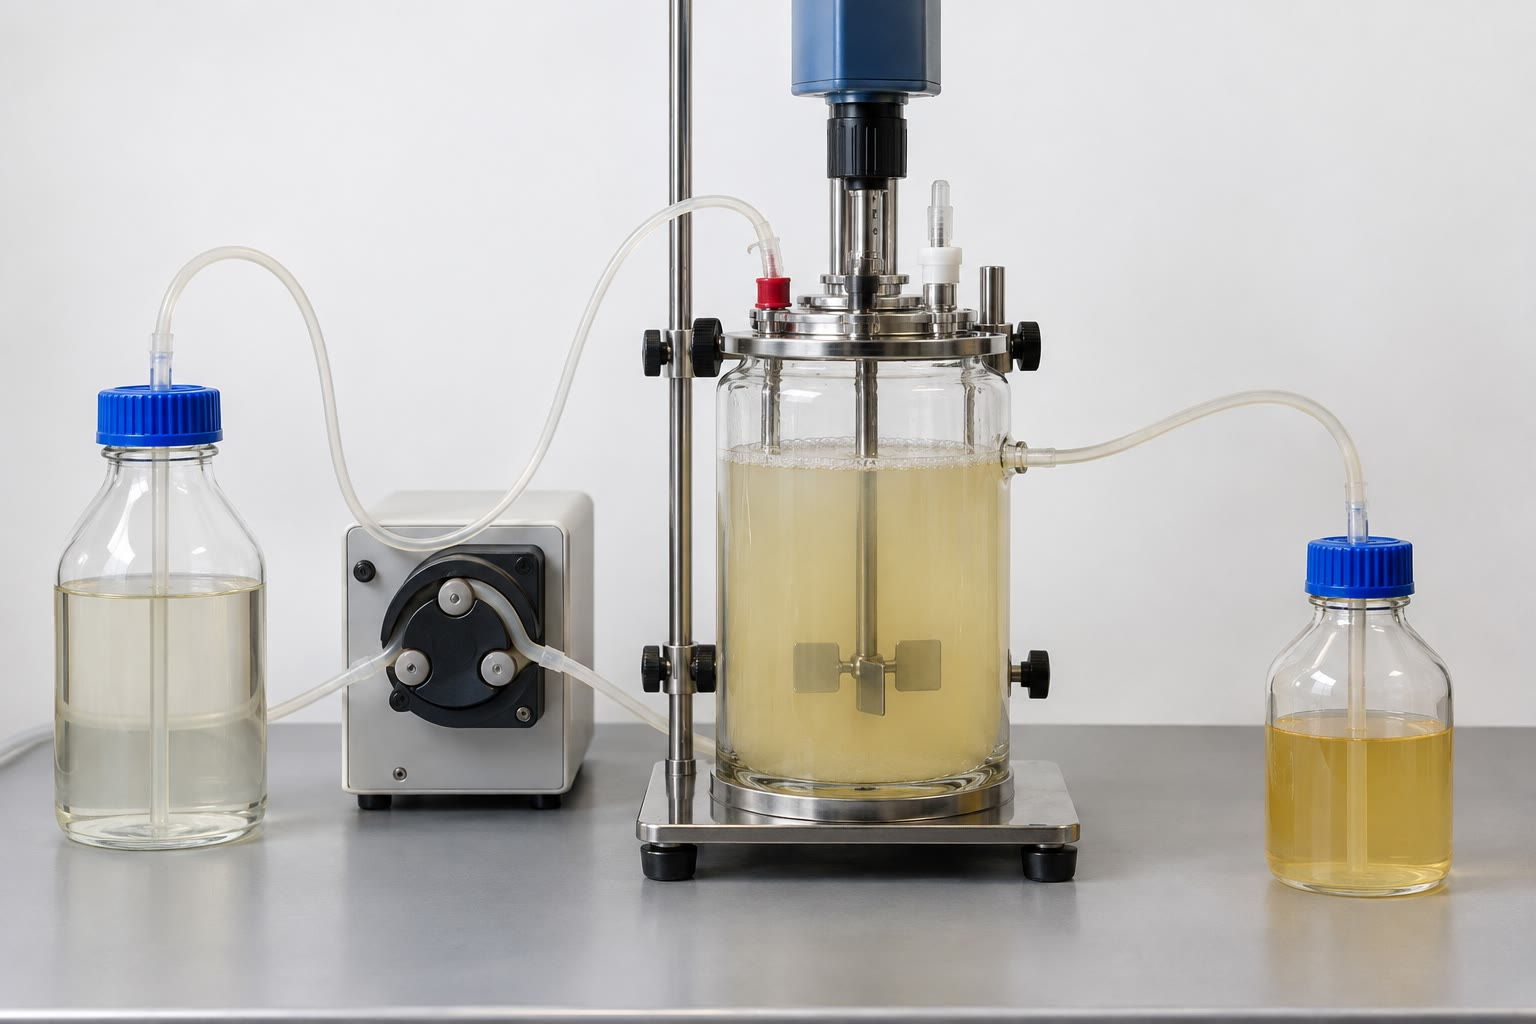
\includegraphics[width=0.6\linewidth]{images/book4/ai/b4-02-chemostat.jpg}

{\small Um quimiostato de laboratório: meio fresco bombeado do
reservatório à esquerda, cultura transbordando à direita; a bomba fixa
a taxa de crescimento.}
\end{omfigure}

\begin{example}[Como ler um quimiostato]\label{ex:b2:microbial-metabolism:chemostat}
Com $\mu_{\max} = \qty{1.0}{h^{-1}}$, $K_s = \qty{0.02}{g/L}$,
$S_{\text{ent}} = \qty{2}{g/L}$ e $Y = 0.5$, a $D =
\qty{0.5}{h^{-1}}$: $S^* = 0.02\times 0.5/0.5 = \qty{0.02}{g/L}$ e
$X^* = 0.5\times 1.98 = \qty{0.99}{g/L}$; a cultura deixa
\qty{1}{\%} do açúcar sem uso. A taxa de lavagem é $1.0\times
2/2.02 = \qty{0.99}{h^{-1}}$. Um biodigestor ou um intestino funciona
pelo mesmo princípio: o cólon humano, alimentado três vezes por dia e
esvaziado uma vez, mantém suas bactérias a uma \omterm{thm:b2:microbial-metabolism:chemostat}{taxa de diluição}
próxima de \qty{0.04}{h^{-1}}, e toda espécie incapaz de se duplicar
em um dia é lavada --- a menos que se prenda à parede.
\end{example}

\section{Biofilmes}

\begin{definition}[Biofilme]\label{def:b2:microbial-metabolism:biofilm}
\index{biofilme}\index{matriz extracelular!bacteriana}
Um \emph{biofilme} é uma comunidade de microrganismos presa a uma
superfície e imersa numa \emph{matriz} que ela mesma produz, feita de
polissacarídeos, proteínas e DNA extracelular. Forma-se em etapas:
\emph{adesão} reversível de células isoladas (flagelos, pili), adesão
irreversível e crescimento de \emph{microcolônias}, \emph{maturação}
num filme estruturado com torres e canais de água, e
\emph{dispersão} de células que saem nadando para colonizar novas
superfícies. A matriz retém água e nutrientes, protege as células da
dessecação, dos predadores, dos antibióticos e das células imunes, e
cria gradientes químicos que fazem do filme uma paisagem de nichos. A
maioria das bactérias da Terra vive assim: sobre as rochas dos
riachos, nas raízes, nos dentes (a placa bacteriana), em cateteres e
implantes, nos pulmões de pacientes com fibrose cística, em cascos de
navios e em tubulações.
\end{definition}

\begin{omfigure}
\begin{tikzpicture}[every node/.style={font=\scriptsize}]
  \fill[gray!35] (0,0) rectangle (13.6,0.35);
  \node at (6.8,0.17) {superfície};
  % stage 1 attachment
  \foreach \p in {(0.6,0.55),(1.4,0.55)} \draw[thick, omDef, fill=omDef!30] \p ellipse (0.22 and 0.1);
  \draw[thick, omDef, fill=omDef!30] (1.0,1.6) ellipse (0.22 and 0.1);
  \draw[->, omDef] (1.0,1.45) -- (1.0,0.75);
  \node[below, align=center] at (1.1,-0.05) {1. adesão};
  % stage 2 microcolony
  \begin{scope}[xshift=3.4cm]
    \fill[omExo!25] (0.15,0.35) .. controls (0.1,1.1) and (1.5,1.1) .. (1.45,0.35);
    \foreach \p in {(0.45,0.5),(0.8,0.5),(1.15,0.5),(0.6,0.75),(0.95,0.75),(0.8,0.95)} \draw[thick, omDef, fill=omDef!30] \p ellipse (0.18 and 0.09);
    \node[below, align=center] at (0.8,-0.05) {2. microcolônia,\\secreção da matriz};
  \end{scope}
  % stage 3 mature with channels
  \begin{scope}[xshift=6.8cm]
    \fill[omExo!25] (0.0,0.35) .. controls (0.2,1.9) and (0.9,2.2) .. (1.1,1.5) .. controls (1.2,0.9) and (1.4,0.6) .. (1.5,0.35);
    \fill[omExo!25] (1.7,0.35) .. controls (1.6,1.5) and (2.6,2.3) .. (2.9,1.2) .. controls (3.0,0.8) and (3.1,0.5) .. (3.2,0.35);
    \foreach \p in {(0.35,0.55),(0.7,0.55),(0.5,0.85),(0.8,1.15),(0.55,1.45),(2.0,0.6),(2.4,0.6),(2.2,0.9),(2.5,1.25),(2.3,1.6),(2.6,1.9),(2.1,1.3)} \draw[thick, omDef, fill=omDef!30] \p ellipse (0.16 and 0.08);
    \draw[<->, omThm, thick] (1.6,0.5) -- (1.6,1.6);
    \node[omThm, anchor=south] at (1.6,2.45) {canal de água};
    \node[below, align=center] at (1.6,-0.05) {3. filme maduro: torres,\\canais, gradientes};
  \end{scope}
  % stage 4 dispersal
  \begin{scope}[xshift=11.2cm]
    \fill[omExo!25] (0.0,0.35) .. controls (0.1,1.5) and (1.0,1.6) .. (1.1,0.35);
    \foreach \p in {(0.3,0.55),(0.65,0.55),(0.5,0.85)} \draw[thick, omDef, fill=omDef!30] \p ellipse (0.16 and 0.08);
    \foreach \p/\a in {(1.4,1.5)/40,(1.9,1.1)/10,(1.6,2.0)/70} \draw[thick, omDef, fill=omDef!30, rotate around={\a:\p}] \p ellipse (0.16 and 0.08);
    \draw[->, omDef] (1.0,1.0) -- (1.35,1.35);
    \node[below, align=center] at (1.0,-0.05) {4. dispersão};
  \end{scope}
\end{tikzpicture}

{\small O ciclo de vida de um \omterm{def:b2:microbial-metabolism:biofilm}{biofilme}: células isoladas aderem,
crescem em microcolônias que secretam uma matriz (cinza),
amadurecem num filme estruturado com torres e canais de água, e
liberam células nadadoras que colonizam novas superfícies.}
\end{omfigure}

\begin{omfigure}
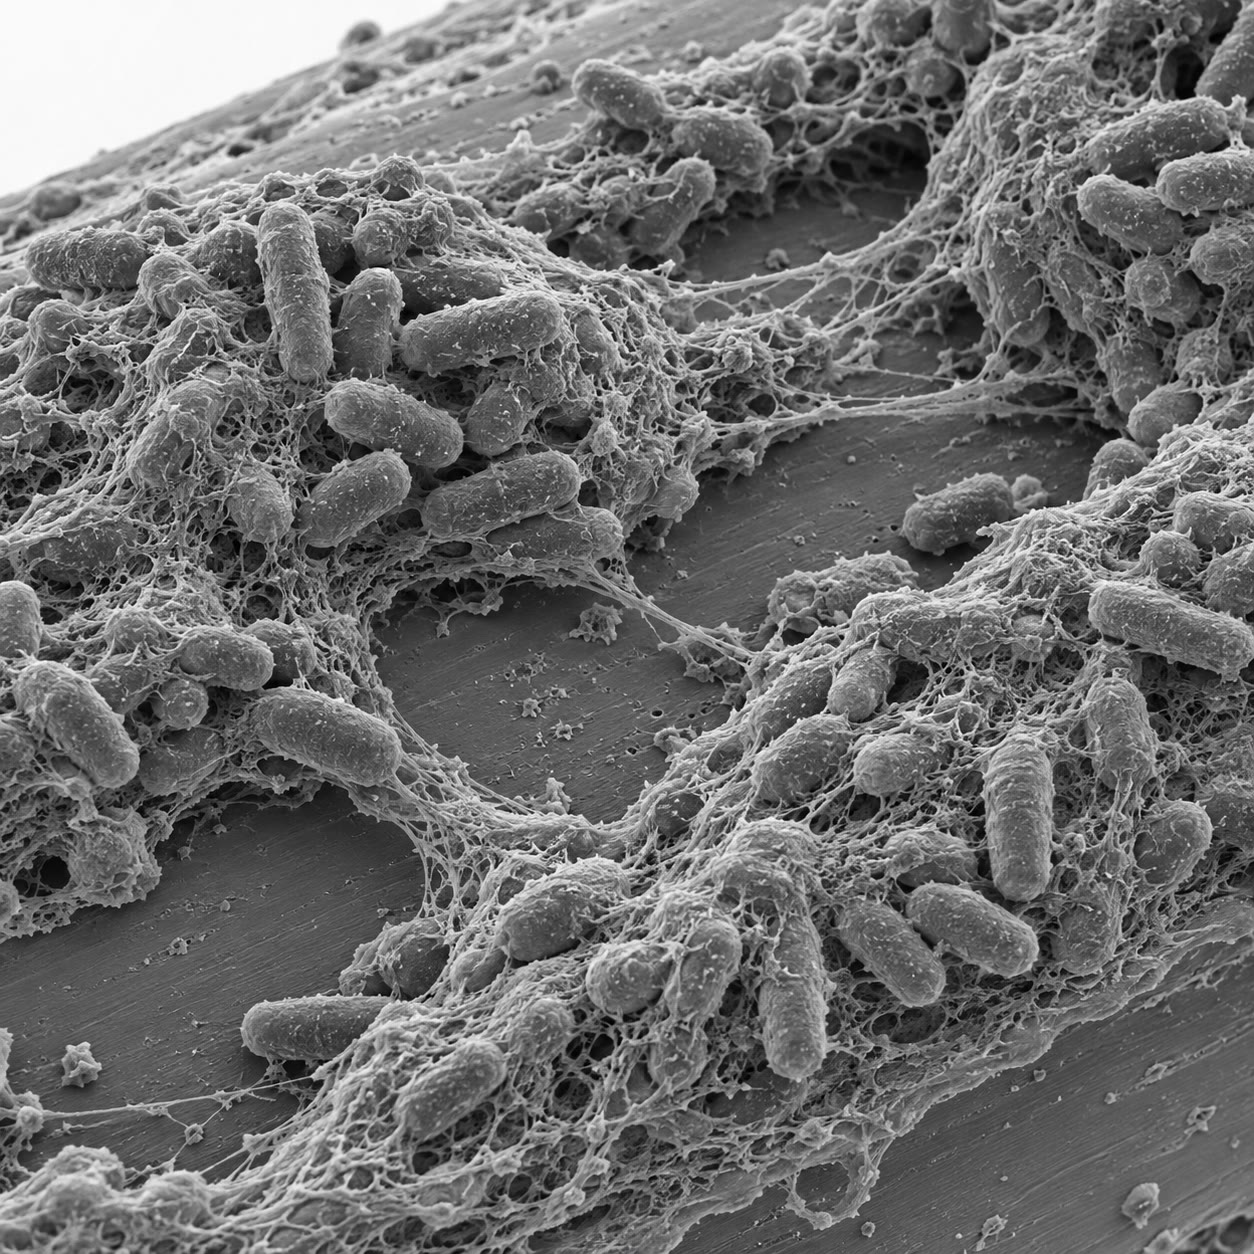
\includegraphics[width=0.46\linewidth]{images/book4/ai/b4-02-biofilm-sem.jpg}

{\small Um \omterm{def:b2:microbial-metabolism:biofilm}{biofilme} sobre um cateter, visto em microscopia eletrônica
de varredura: bactérias em bastonete imersas na matriz fibrosa que
secretaram, com canais abertos entre os aglomerados.}
\end{omfigure}

\begin{theorem}[Gradientes no interior de um biofilme]\label{thm:b2:microbial-metabolism:gradient}
\index{profundidade de penetração do oxigênio}
Num filme de espessura $L$ cujas células consomem oxigênio a uma taxa
volumétrica constante $q$, com a concentração mantida em $c_0$ na
superfície e nenhum fluxo através do substrato de fixação, o perfil
estacionário de oxigênio é uma parábola e, se o filme for espesso o
bastante para o oxigênio se esgotar, isso ocorre na
\emph{profundidade de penetração}
\[
L_p = \sqrt{\frac{2 D_e\, c_0}{q}},
\]
em que $D_e$ é o coeficiente de difusão efetivo na matriz.
Com $D_e = \qty{1.5e-9}{m^2/s}$, $c_0 = \qty{0.25}{mol/m^3}$ e $q
= \qty{0.17}{mol/m^3/s}$ (um filme denso de células que respiram), $L_p
\approx \qty{66}{\micro m}$: abaixo de um décimo de milímetro, um
\omterm{def:b2:microbial-metabolism:biofilm}{biofilme} é anóxico, e desnitrificantes, fermentadores e redutores de
sulfato vivem sob um teto de aeróbios.
\end{theorem}
\begin{proof}
Seja $x$ a profundidade abaixo da superfície. Em regime estacionário, o
fluxo difusivo $-D_e\,\mathrm{d}c/\mathrm{d}x$ varia com a
profundidade apenas pelo consumo: $D_e\,\mathrm{d}^2c/\mathrm{d}x^2 = q$.
Integrando duas vezes, $c = c_0 + a x + q x^2/2D_e$. Se o oxigênio se
anula na profundidade $L_p$ com fluxo nulo ali (nada chega de baixo),
$c(L_p) = 0$ e $c'(L_p) = 0$: a segunda condição dá $a = -qL_p/D_e$,
e a primeira dá então $c_0 - qL_p^2/D_e + qL_p^2/2D_e = 0$, isto é,
$L_p^2 = 2D_e c_0/q$. O perfil é $c = (q/2D_e)(L_p - x)^2$.
\end{proof}

\begin{omfigure}
\begin{tikzpicture}
\begin{axis}[
  width=0.78\linewidth, height=5.6cm,
  axis x line=bottom, axis y line=left,
  xmin=0, xmax=120, ymin=0, ymax=0.28,
  xlabel={profundidade no filme (\unit{\micro m})}, ylabel={$\mathrm{O_2}$ (\unit{mol/m^3})},
  xlabel style={font=\small, at={(axis description cs:0.5,-0.14)}, anchor=north},
  ylabel style={font=\small},
  tick label style={font=\small}, xtick={0,20,40,60,80,100,120}, ytick={0,0.1,0.2},
  clip=false,
]
\addplot[very thick, omDef, domain=0:66, samples=60] {0.25*(1-x/66)^2};
\addplot[very thick, omDef, domain=66:120, samples=2] {0};
\fill[omThm!12] (axis cs:66,0) rectangle (axis cs:120,0.28);
\node[font=\scriptsize, anchor=north, align=center] at (axis cs:93,0.27) {zona anóxica:\\desnitrificantes, fermentadores,\\redutores de sulfato};
\draw[dashed, gray] (axis cs:66,0) -- (axis cs:66,0.28); \node[font=\scriptsize, anchor=south] at (axis cs:66,0.28) {$L_p$};
\node[font=\scriptsize, anchor=west] at (axis cs:24,0.18) {zona aeróbia};
\end{axis}
\end{tikzpicture}

{\small O oxigênio no interior de um \omterm{def:b2:microbial-metabolism:biofilm}{biofilme} que respira: uma queda
parabólica do valor do meio na superfície até zero na profundidade de
penetração, \qty{66}{\micro m} para os valores do teorema. Tudo o que
fica mais fundo é anóxico.}
\end{omfigure}

\begin{proposition}[Percepção de quórum]\label{prop:b2:microbial-metabolism:quorum}
\index{percepção de quórum}\index{autoindutor}
As bactérias contam a si mesmas (\textit{quorum sensing}). Cada célula secreta, a uma taxa baixa
e constante, uma pequena molécula sinalizadora, um
\emph{autoindutor} (lactonas de acil-homosserina nas Gram-negativas,
peptídeos curtos nas Gram-positivas). Numa suspensão diluída, o sinal
se dispersa por difusão; numa população densa ou num \omterm{def:b2:microbial-metabolism:biofilm}{biofilme}, ele se
acumula e, acima de uma concentração limiar, liga-se a um receptor que
ativa um conjunto de genes --- inclusive o gene do próprio autoindutor,
daí o nome. Os genes assim controlados são aqueles que só compensam
quando muitas células agem juntas: a luminescência, a secreção de
enzimas digestivas e de toxinas, a produção da matriz, a virulência de
patógenos que precisam dominar um hospedeiro de uma só vez em vez de
alertá-lo célula por célula.
\end{proposition}
\begin{proof}[Evidências]
Nealson, Platt e Hastings (1970) verificaram que a bactéria marinha
\emph{Vibrio fischeri}, que ilumina o órgão luminoso de uma lula, é
escura em cultura diluída e só brilha acima de cerca de $10^{7}$
células por mililitro; o meio livre de células, retirado de uma
cultura densa e luminosa, fazia uma cultura diluída brilhar
imediatamente. O meio continha o sinal; sua estrutura, uma lactona de
acil-homosserina, foi determinada em 1981, e mutantes incapazes de
produzi-la nunca brilham, por mais densos que se tornem.
\end{proof}

\begin{example}[Por que um biofilme sobrevive aos antibióticos]\label{ex:b2:microbial-metabolism:tolerance}
As células de um \omterm{def:b2:microbial-metabolism:biofilm}{biofilme} sobrevivem a concentrações de antibiótico
cem a mil vezes maiores que as que matam a mesma linhagem em
suspensão, sem nenhum gene de resistência. A matriz retarda a difusão
do fármaco e retém parte dele; os gradientes deixam as células
profundas famintas, anóxicas e quase sem crescer, e a maioria dos
antibióticos só mata células em crescimento (as penicilinas precisam
da síntese da parede, os aminoglicosídeos precisam de transporte
ativo); algumas células \emph{persistentes} estão totalmente dormentes
e reconstituem o filme quando o tratamento para. Uma infecção crônica
sobre um implante é, por isso, geralmente tratada com a remoção do
implante.
\end{example}

\section{Comunidades microbianas}

\begin{example}[A coluna de Winogradsky explicada]\label{ex:b2:microbial-metabolism:column}
A luz e o ar entram por cima; a matéria orgânica e o sulfato vêm da
lama. Cianobactérias e algas crescem no topo e liberam oxigênio. Mais
abaixo, os heterótrofos esgotam o oxigênio sobre a matéria orgânica,
depois o nitrato; mais fundo, os redutores de sulfato transformam o
sulfato em sulfeto, que se difunde para cima e enegrece a lama com
sulfeto de ferro. Onde o sulfeto que sobe encontra a luz que desce, as
bactérias sulfurosas púrpuras o oxidam pela fotossíntese (a faixa
púrpura), com as bactérias sulfurosas verdes logo abaixo; onde o
sulfeto encontra o oxigênio, no escuro, oxidantes de enxofre incolores
como \emph{Beggiatoa} ganham a vida pela \omterm{def:b2:microbial-metabolism:trophic}{quimiolitotrofia} (o véu
branco); onde o ferro reduzido encontra o oxigênio, os oxidantes de
ferro deixam uma faixa cor de ferrugem. O enxofre circula entre sulfeto
e sulfato dentro da coluna; o carbono, entre o
$\mathrm{CO_2}$ e a matéria orgânica; só a luz entra e só o calor
sai. É um ecossistema fechado com um balanço energético aberto, e um
modelo em escala do fundo do oceano.
\end{example}

\begin{omfigure}
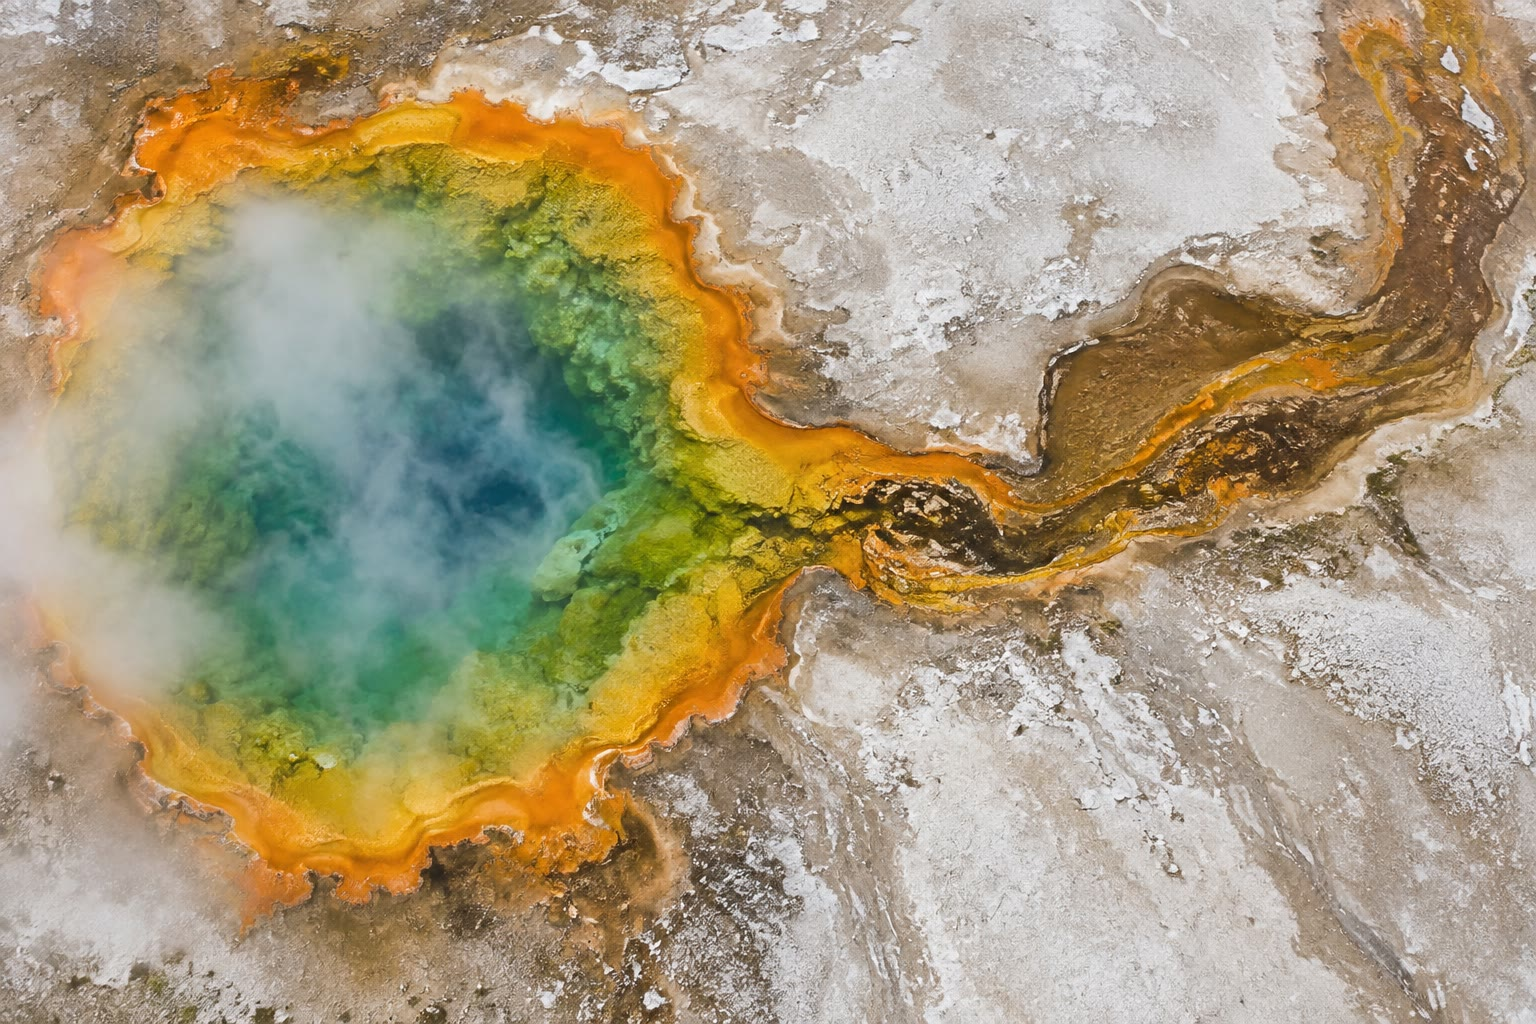
\includegraphics[width=0.62\linewidth]{images/book4/ai/b4-02-hot-spring-mats.jpg}

{\small Tapetes microbianos em torno de uma fonte termal: cada cor é
uma população que vive na temperatura e na química de sua faixa ---
cianobactérias termófilas e bactérias verdes no escoamento mais frio,
\omterm{def:b2:microbial-metabolism:trophic}{quimiolitotróficos} incolores na água mais quente.}
\end{omfigure}

\begin{remark}[Os tapetes microbianos e a Terra primitiva]\label{rem:b2:microbial-metabolism:mats}
Em torno de fontes termais e em planícies de maré, tapetes microbianos
estratificados de alguns milímetros de espessura concentram a coluna
inteira numa espessura que a luz consegue atravessar: cianobactérias
em cima, bactérias púrpuras embaixo, redutores de sulfato na base, cada
camada consumindo o que a de cima produz, e o tapete migrando para
cima através do sedimento que retém. Os tapetes fósseis --- os
estromatólitos --- são a mais antiga evidência de vida, com
\num{3.5} bilhões de anos. Durante dois bilhões de anos, antes das
plantas e dos animais, a biosfera foi esses tapetes e o plâncton
acima deles, e foram eles que encheram o ar de oxigênio
(\cref{ch:b2:biogeochemical-cycles}).
\end{remark}

\section{Exercícios}

\begin{exercise}[$\star$]\label{exo:b2:microbial-metabolism:1}
Classifique segundo a fonte de energia, a fonte de elétrons e a fonte
de carbono: uma cianobactéria; \emph{Nitrosomonas}; \emph{E.~coli} em
glicose; uma bactéria púrpura não sulfurosa que cresce na luz sobre
succinato; \emph{Thiobacillus} sobre $\mathrm{H_2S}$ no escuro.
\end{exercise}

\begin{exercise}[$\star$]\label{exo:b2:microbial-metabolism:2}
Liste os aceptores de elétrons da respiração em ordem decrescente de
rendimento energético, e diga em que ponto de um sedimento cada um é
usado.
\end{exercise}

\begin{exercise}[$\star$]\label{exo:b2:microbial-metabolism:3}
Balanceie a oxidação da glicose a $\mathrm{CO_2}$ pelo nitrato
reduzido a $\mathrm{N_2}$ (em solução ácida, com água como o outro
produto). Quantos íons nitrato por glicose?
\end{exercise}

\begin{exercise}[$\star$]\label{exo:b2:microbial-metabolism:4}
Defina \omterm{def:b2:microbial-metabolism:biofilm}{biofilme} e cite suas quatro etapas. Dê três situações em que os
\omterm{def:b2:microbial-metabolism:biofilm}{biofilmes} importam para a saúde humana ou para a indústria.
\end{exercise}

\begin{exercise}[$\star\star$]\label{exo:b2:microbial-metabolism:5}
Calcule $\Delta G^{\circ\prime}$ para $4\mathrm{H_2} + \mathrm{CO_2}
\to \mathrm{CH_4} + 2\mathrm{H_2O}$ a partir dos potenciais
$\mathrm{2H^+/H_2}$ (\qty{-0.42}{V}) e $\mathrm{CO_2/CH_4}$
(\qty{-0.24}{V}). Quantos ATP (a \qty{50}{kJ/mol}) um metanogênico
pode produzir, no máximo, por $\mathrm{H_2}$? Comente sua taxa de
crescimento.
\end{exercise}

\begin{exercise}[$\star\star$]\label{exo:b2:microbial-metabolism:6}
Uma bactéria tem $\mu_{\max} = \qty{1.2}{h^{-1}}$ e $K_s =
\qty{5}{mg/L}$ de glicose. Calcule $\mu$ e o \omterm{def:b2:unicellular-diversity:division}{tempo de geração} a
1, 5 e \qty{50}{mg/L}. Em que concentração ela cresce a
\qty{90}{\%} de seu máximo?
\end{exercise}

\begin{exercise}[$\star\star$]\label{exo:b2:microbial-metabolism:7}
Um quimiostato com $\mu_{\max} = \qty{0.8}{h^{-1}}$, $K_s =
\qty{0.05}{g/L}$, $S_{\text{ent}} = \qty{5}{g/L}$, $Y = 0.4$ opera a
$D = \qty{0.4}{h^{-1}}$. Calcule $S^*$, $X^*$, a produção de biomassa
por litro por hora e a taxa de lavagem.
\end{exercise}

\begin{exercise}[$\star\star$]\label{exo:b2:microbial-metabolism:8}
A oxidação de um $\mathrm{NH_4^+}$ a nitrito fornece \qty{275}{kJ};
uma nitrificante captura um quarto disso como ATP (\qty{50}{kJ/mol}),
e fixar um $\mathrm{CO_2}$ em biomassa custa o equivalente a 12
ATP. Quantos íons amônio ela precisa oxidar por carbono fixado? Por que
o rendimento de uma nitrificante é tão baixo comparado ao de um
heterótrofo?
\end{exercise}

\begin{exercise}[$\star\star$]\label{exo:b2:microbial-metabolism:9}
Calcule a \omterm{thm:b2:microbial-metabolism:gradient}{profundidade de penetração do oxigênio} num \omterm{def:b2:microbial-metabolism:biofilm}{biofilme} com
$D_e =
\qty{1.2e-9}{m^2/s}$, $c_0 = \qty{0.20}{mol/m^3}$ e $q =
\qty{0.5}{mol/m^3/s}$. O que acontece com $L_p$ se o oxigênio do meio
dobrar? E se as células respirarem quatro vezes mais depressa?
\end{exercise}

\begin{exercise}[$\star\star\star$]\label{exo:b2:microbial-metabolism:10}
Preveja as faixas de uma coluna de Winogradsky de cima para baixo,
indicando o metabolismo de cada uma, e explique (a) por que a faixa
púrpura se forma onde se forma, (b) por que a lama fica negra, (c) em
que sentido a coluna é um sistema fechado e em que sentido é aberto.
\end{exercise}

\begin{exercise}[$\star\star\star$]\label{exo:b2:microbial-metabolism:11}
Cada célula de uma população de densidade $n$ (células por litro)
secreta um autoindutor a $p = 5$ moléculas por segundo; a molécula é
degradada a uma taxa $k = \qty{5e-4}{s^{-1}}$. Escreva a concentração
estacionária $A^*$ em função de $n$. O receptor é ativado a
$A_c = \qty{10}{nmol/L}$: calcule a densidade limiar em células por
mililitro. Compare com uma cultura densa ($10^{9}$ por mililitro) e
com a água do mar ($10^{5}$ por mililitro), e explique por que um
\omterm{def:b2:microbial-metabolism:biofilm}{biofilme} atinge o quórum num volume em que uma suspensão nunca o
atingiria.
\end{exercise}

\begin{exercise}[$\star\star\star$]\label{exo:b2:microbial-metabolism:12}
``Os \omterm{def:b2:unicellular-diversity:prokaryote}{procariotos} comandam a química do planeta.'' Discuta com base em
três processos deste capítulo que nenhum eucarioto é capaz de
realizar, dizendo para cada um o que aconteceria com a biosfera se ele
parasse.
\end{exercise}

\section{Problema: Uma estação de tratamento de esgoto}

\begin{problem}[{Problema de fim de semana --- o tratamento de esgoto
de uma cidade analisado como um conjunto de reatores microbianos, da
energética de suas bactérias ao metano que o abastece, até o balanço
energético da estação}]
\label{pb:b2:microbial-metabolism:1}
Uma estação trata $Q = \qty{10000}{m^3}$ de esgoto por dia, com
\qty{300}{g/m^3} de matéria orgânica, medida pelo oxigênio necessário
para queimá-la (sua \emph{demanda química de oxigênio}, DQO), e
\qty{40}{g/m^3} de nitrogênio amoniacal. Ela tem um tanque aerado de
lodo ativado, um tanque anóxico para a \omterm{def:b2:microbial-metabolism:anaerobic}{desnitrificação} e um digestor
anaeróbio para o lodo. Dados: os heterótrofos aeróbios convertem a
matéria orgânica com um rendimento $Y = 0.4$ (quilograma de DQO de
biomassa por quilograma de DQO de substrato; o restante é oxidado);
a nitrificação exige \qty{4.57}{kg} de $\mathrm{O_2}$ por quilograma de
nitrogênio; a \omterm{def:b2:microbial-metabolism:anaerobic}{desnitrificação} exige \qty{2.86}{kg} de DQO de substrato
por quilograma de nitrogênio de nitrato; a aeração fornece \qty{2}{kg}
de $\mathrm{O_2}$ por quilowatt-hora; a DQO do lodo é convertida em
metano no digestor a \qty{60}{\%}, cada quilograma de DQO convertido
dando \qty{0.35}{m^3} de metano de conteúdo energético
\qty{36}{MJ/m^3}, queimado num gerador de \qty{35}{\%} de eficiência
elétrica. Nitrificantes: $\mu_{\max} = \qty{0.5}{d^{-1}}$, $K_s =
\qty{1}{g/m^3}$ de nitrogênio amoniacal.

\medskip
\noindent\textbf{Parte I --- A energética.}
\begin{enumerate}
  \item Usando a \omterm{thm:b2:microbial-metabolism:redox}{torre de elétrons}, calcule $\Delta G^{\circ\prime}$
        para a oxidação de um mol de glicose (24 elétrons a
        \qty{-0.43}{V}) pelo oxigênio (\qty{+0.82}{V}).
  \item Calcule-o para o nitrato reduzido a $\mathrm{N_2}$
        (\qty{+0.74}{V}) e para o sulfato reduzido a sulfeto
        (\qty{-0.22}{V}).
  \item Por que a \omterm{def:b2:microbial-metabolism:anaerobic}{desnitrificação} só começa no tanque anóxico, e por
        que a \omterm{def:b2:microbial-metabolism:anaerobic}{redução do sulfato} (com seu cheiro) é sinal de uma
        estação mal operada?
  \item Se as células capturam \qty{40}{\%} da energia livre como ATP
        (\qty{50}{kJ/mol}), quantos ATP por glicose fornece cada um dos
        três metabolismos?
  \item Quanto mais glicose um redutor de sulfato precisa processar,
        em relação a um aeróbio, para o mesmo crescimento?
  \item Os fermentadores do digestor obtêm 2 ATP por glicose. Explique
        por que, ainda assim, o digestor produz quase nenhuma biomassa
        e sobretudo gás.
\end{enumerate}

\medskip
\noindent\textbf{Parte II --- O tanque aerado.}
\begin{enumerate}[resume]
  \item Calcule a carga diária de matéria orgânica, em quilogramas de
        DQO.
  \item Calcule a biomassa produzida por dia (em DQO) e o oxigênio
        necessário para oxidar o restante.
  \item Calcule a energia de aeração para a matéria orgânica, em
        quilowatts-hora por dia.
  \item Calcule a carga diária de nitrogênio e o oxigênio necessário
        para nitrificá-la.
  \item O lodo fica retido no tanque por um tempo médio $\theta$
        (o inverso de sua \omterm{thm:b2:microbial-metabolism:chemostat}{taxa de diluição}). Abaixo de que $\theta$ as
        nitrificantes são lavadas, qualquer que seja a concentração de
        amônio?
  \item Com $\theta = \qty{10}{d}$, calcule a concentração residual
        de amônio no efluente.
  \item O inverno reduz $\mu_{\max}$ a \qty{0.25}{d^{-1}}. Recalcule
        o amônio residual e diga o que o operador deve fazer.
\end{enumerate}

\medskip
\noindent\textbf{Parte III --- A \omterm{def:b2:microbial-metabolism:anaerobic}{desnitrificação} e o digestor.}
O nitrato produzido no tanque aerado é recirculado para o tanque
anóxico, onde heterótrofos o reduzem com a matéria orgânica que chega.
\begin{enumerate}[resume]
  \item Calcule a matéria orgânica (quilogramas de DQO por dia)
        consumida na \omterm{def:b2:microbial-metabolism:anaerobic}{desnitrificação} de todo o nitrogênio.
  \item Calcule a massa de nitrogênio liberada para o ar como
        $\mathrm{N_2}$ por dia, e a massa que sai no efluente
        como amônio (questão 12), como fração da carga.
  \item Essa matéria orgânica deixa de precisar de aeração. Calcule o
        oxigênio economizado e a demanda total de oxigênio da estação
        (matéria orgânica restante mais nitrificação).
  \item O lodo produzido (questão 8, contado como DQO) vai para o
        digestor. Calcule o metano produzido por dia.
  \item Calcule a energia desse metano e a eletricidade que ele
        fornece.
  \item Calcule a eletricidade de aeração para a demanda total de
        oxigênio da questão 16, e compare.
\end{enumerate}

\medskip
\noindent\textbf{Parte IV --- O reator de \omterm{def:b2:microbial-metabolism:biofilm}{biofilme}.}
Um filtro biológico percolador cultiva um \omterm{def:b2:microbial-metabolism:biofilm}{biofilme} sobre pedras; a água
contém \qty{0.2}{mol/m^3} de oxigênio, $D_e = \qty{1.5e-9}{m^2/s}$, e
o filme respira a $q = \qty{0.3}{mol/m^3/s}$.
\begin{enumerate}[resume]
  \item Deduza o perfil de oxigênio $c(x)$ num filme espesso o bastante
        para se tornar anóxico.
  \item Calcule a profundidade de penetração.
  \item O filme tem \qty{300}{\micro m} de espessura. Que fração dele é
        aeróbia, e o que as células de baixo fazem com o nitrato que se
        difunde a partir da camada aeróbia?
  \item Explique por que um único \omterm{def:b2:microbial-metabolism:biofilm}{biofilme} consegue nitrificar e
        desnitrificar ao mesmo tempo, o que o tanque aerado não
        consegue.
  \item Adiciona-se cloro para desinfetar o efluente. Dê duas razões
        pelas quais o \omterm{def:b2:microbial-metabolism:biofilm}{biofilme} sobrevive a uma dose que mata as mesmas
        bactérias em suspensão.
  \item Enuncie o resultado: a demanda diária de oxigênio da estação,
        sua produção de metano e a fração da eletricidade de aeração
        que o metano fornece.
\end{enumerate}
\end{problem}
